\apendice{Especificación de diseño}

\section{Introducción}

Este anexo tiene bastante relación con el anterior, ya que trataremos de mostrar la parte de diseño referente al análisis que se ha realizado en anexo 2. 

Para realizar este diseño hablaremos de 3 fases principales:

\begin{itemize}
\item Diseño estructural: se detalla como hemos estructurado todos los datos y recursos que posee la aplicación, con el fin de que tenga una comprensión más sencilla.
\item Diseño procedimental: Se define todos los estados por los que puede pasar la aplicación durante su utilización y en base a las distintas situaciones que puedan surgir.
\item Pruebas: Se reflejará las distintas pruebas que se han realizado sobre la aplicación.
\end{itemize}

\section{Diseño de datos}

En este apartado se hará referencia a cómo están organizados los datos y cada una de 

\subsection{Base de datos geo-espacial}

Debido a que seguimos desarrollando el proyecto a partir de uno anterior, utilizaremos la misma base de datos geoespacial, proporcionada por OpenStreetMaps y con la cual podremos acceder a datos necesarios para el trabajo.

La estructura de la base de datos ha sido modificada ligeramente para que los algoritmos se puedan nutrir de ventanas de tiempo. Para el resto de la estructura de la base de datos, así como el conjunto de tablas, se ha mantenido tal y como estaba. Si es necesario analizar cualquiera de estas partes, será preferible observar la memoria del trabajo anterior a este.

Igualmente, el modelo de datos, las tablas generales y la tabla que almacena las rutas, se mantienen sin cambios.

\subsection{Estructura de paquetes del servidor}

La estructura de paquetes del servidor ha sido la parte de la que se ha encargado mi compañero Ignacio, para la cual ha realizado modificaciones con respecto a lo anterior, aunque manteniendo una estructura general bastante parecida. 

Los cambios más relevantes en esta estructura son los referentes al añadido de nuevos algoritmos de cálculo de rutas y también a la implementación de nuevas estructura con herencia. Estos cambios se pueden ver en las siguientes imágenes que pertenecen al trabajo de mi compañero, por lo que si se quiere información más detallada es preferible visitar su proyecto.

\subsection{Estructura de paquetes del cliente}

Ésta parte tendrá mas detalle que la anterior, ya que este proyecto se ha centrado en la interfaz de la aplicación y por tanto también se han hecho modificaciones en la estructura de paquetes de la misma.

\subsubsection{Paquete activities}

\subsubsection{Paquete adapters}

\subsubsection{Paquete communication}

\subsubsection{Paquete útil}

\subsection{Diagrama de despliegue}

Tal como en el proyecto anterior, haremos referencia al trabajo original a partir del cual se desarrolló este diagrama sobre el funcionamiento a rasgos generales de como se comportan el cliente y el servidor a la hora de enviar y recibir datos entre ellos.

El cliente realiza peticiones del tipo REST hacia el servidor. Para que esa petición pueda avanzar, pasará por un "servlet" y se ejecutará dentro de Glassfish. En este momento será cuando haga falta una consulta de tipo SQL hacia la base de datos, para obtener la información que se solicite.

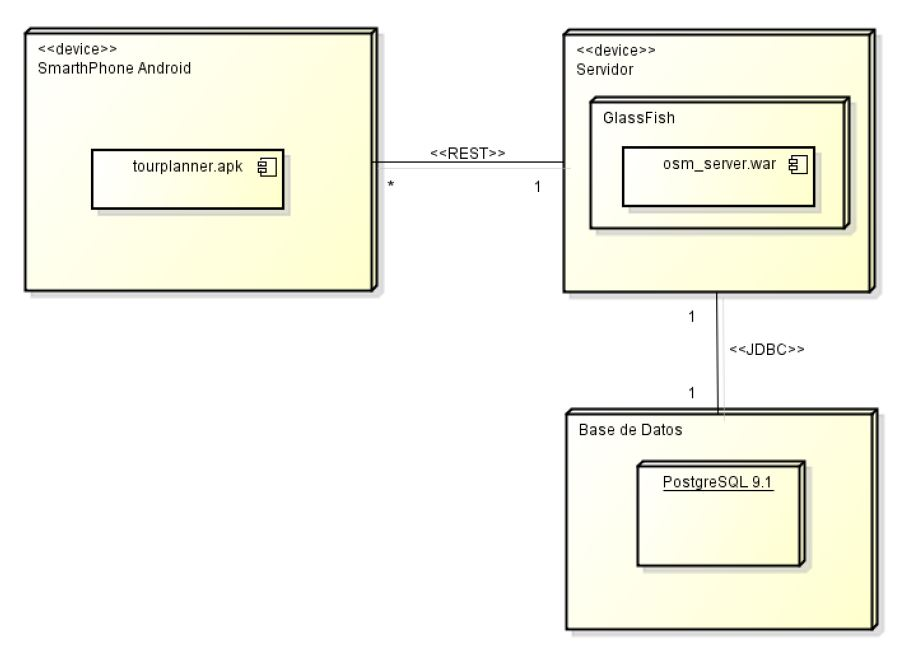
\includegraphics[width=\textwidth]{diagramaDespliegue.jpg}


\section{Diseño procedimental}

\subsection{Diagramas de secuencia}

\section{Diseño arquitectónico}

En este apartado se pueden ver los distintos patrones de diseño que han sido aplicados sobre el código para lograr una estructura mucho mas homogénea y reutilizable a futuro.

Como se comentó en el proyecto anterior, se aplicaron los patrones Singleton y Facade para dos partes distintas del desarrollo de la estructura del proyecto.

Por desgracia, el patrón Facade se implementó para acceder al servicio de Panoramio, el cual ya no se encuentra activo, por lo que objetivamente no se está poniendo en práctica real para este proyecto. De todas formas, es un patrón perfectamente válido y una vez localizada una API que pueda sustituir los servicios prestados por Panoramio, se podría volver a aplicar sin ningún problema.

El patrón Singleton se sigue utilizando para el manejo de la clase SSLFactory, ya que seguimos necesitando validar y asegurar que se está realizando una conexión HTTPS con el servidor y este patrón nos ayuda bastante para poder hacerlo de manera ordenada.


